\subsection*{Velocity}
Det var �benlyst for os at vi i de forrige sprints have vurderet vores velocity for h�jt, s� i sprint 3 vurderede vi den ud fra hvor mange mandetimer vi havde n�et i sprint 2, minus lidt yderligere da vi faktisk havde lavet overarbejde i sprint 2. \\
F�lgende har vi fundet ud af vores velocity var lavere pga. manglende erfaring og teknisk niveau for nogle i gruppen.
Dette resulterer i at vi ikke helt havde ressourcerne for to hold, men n�rmere 1,5 p� en god dag. Vi forventer at have 4 mandetimer om dagen per mand i gruppen, dvs. 6 mandetimer om dagen med 1,5 hold.\\
I alt forventede vi at have 16 mandetimer i sprintet med 3 dage, efter at have tr�kke yderligere 2 mandetimer fra for at skabe yderligere rum: \\
16 mandetimer * 0,625 = 10 story points per uge, dvs. 3,33 story points per dag.

\begin{figure}[H]
\begin{center}
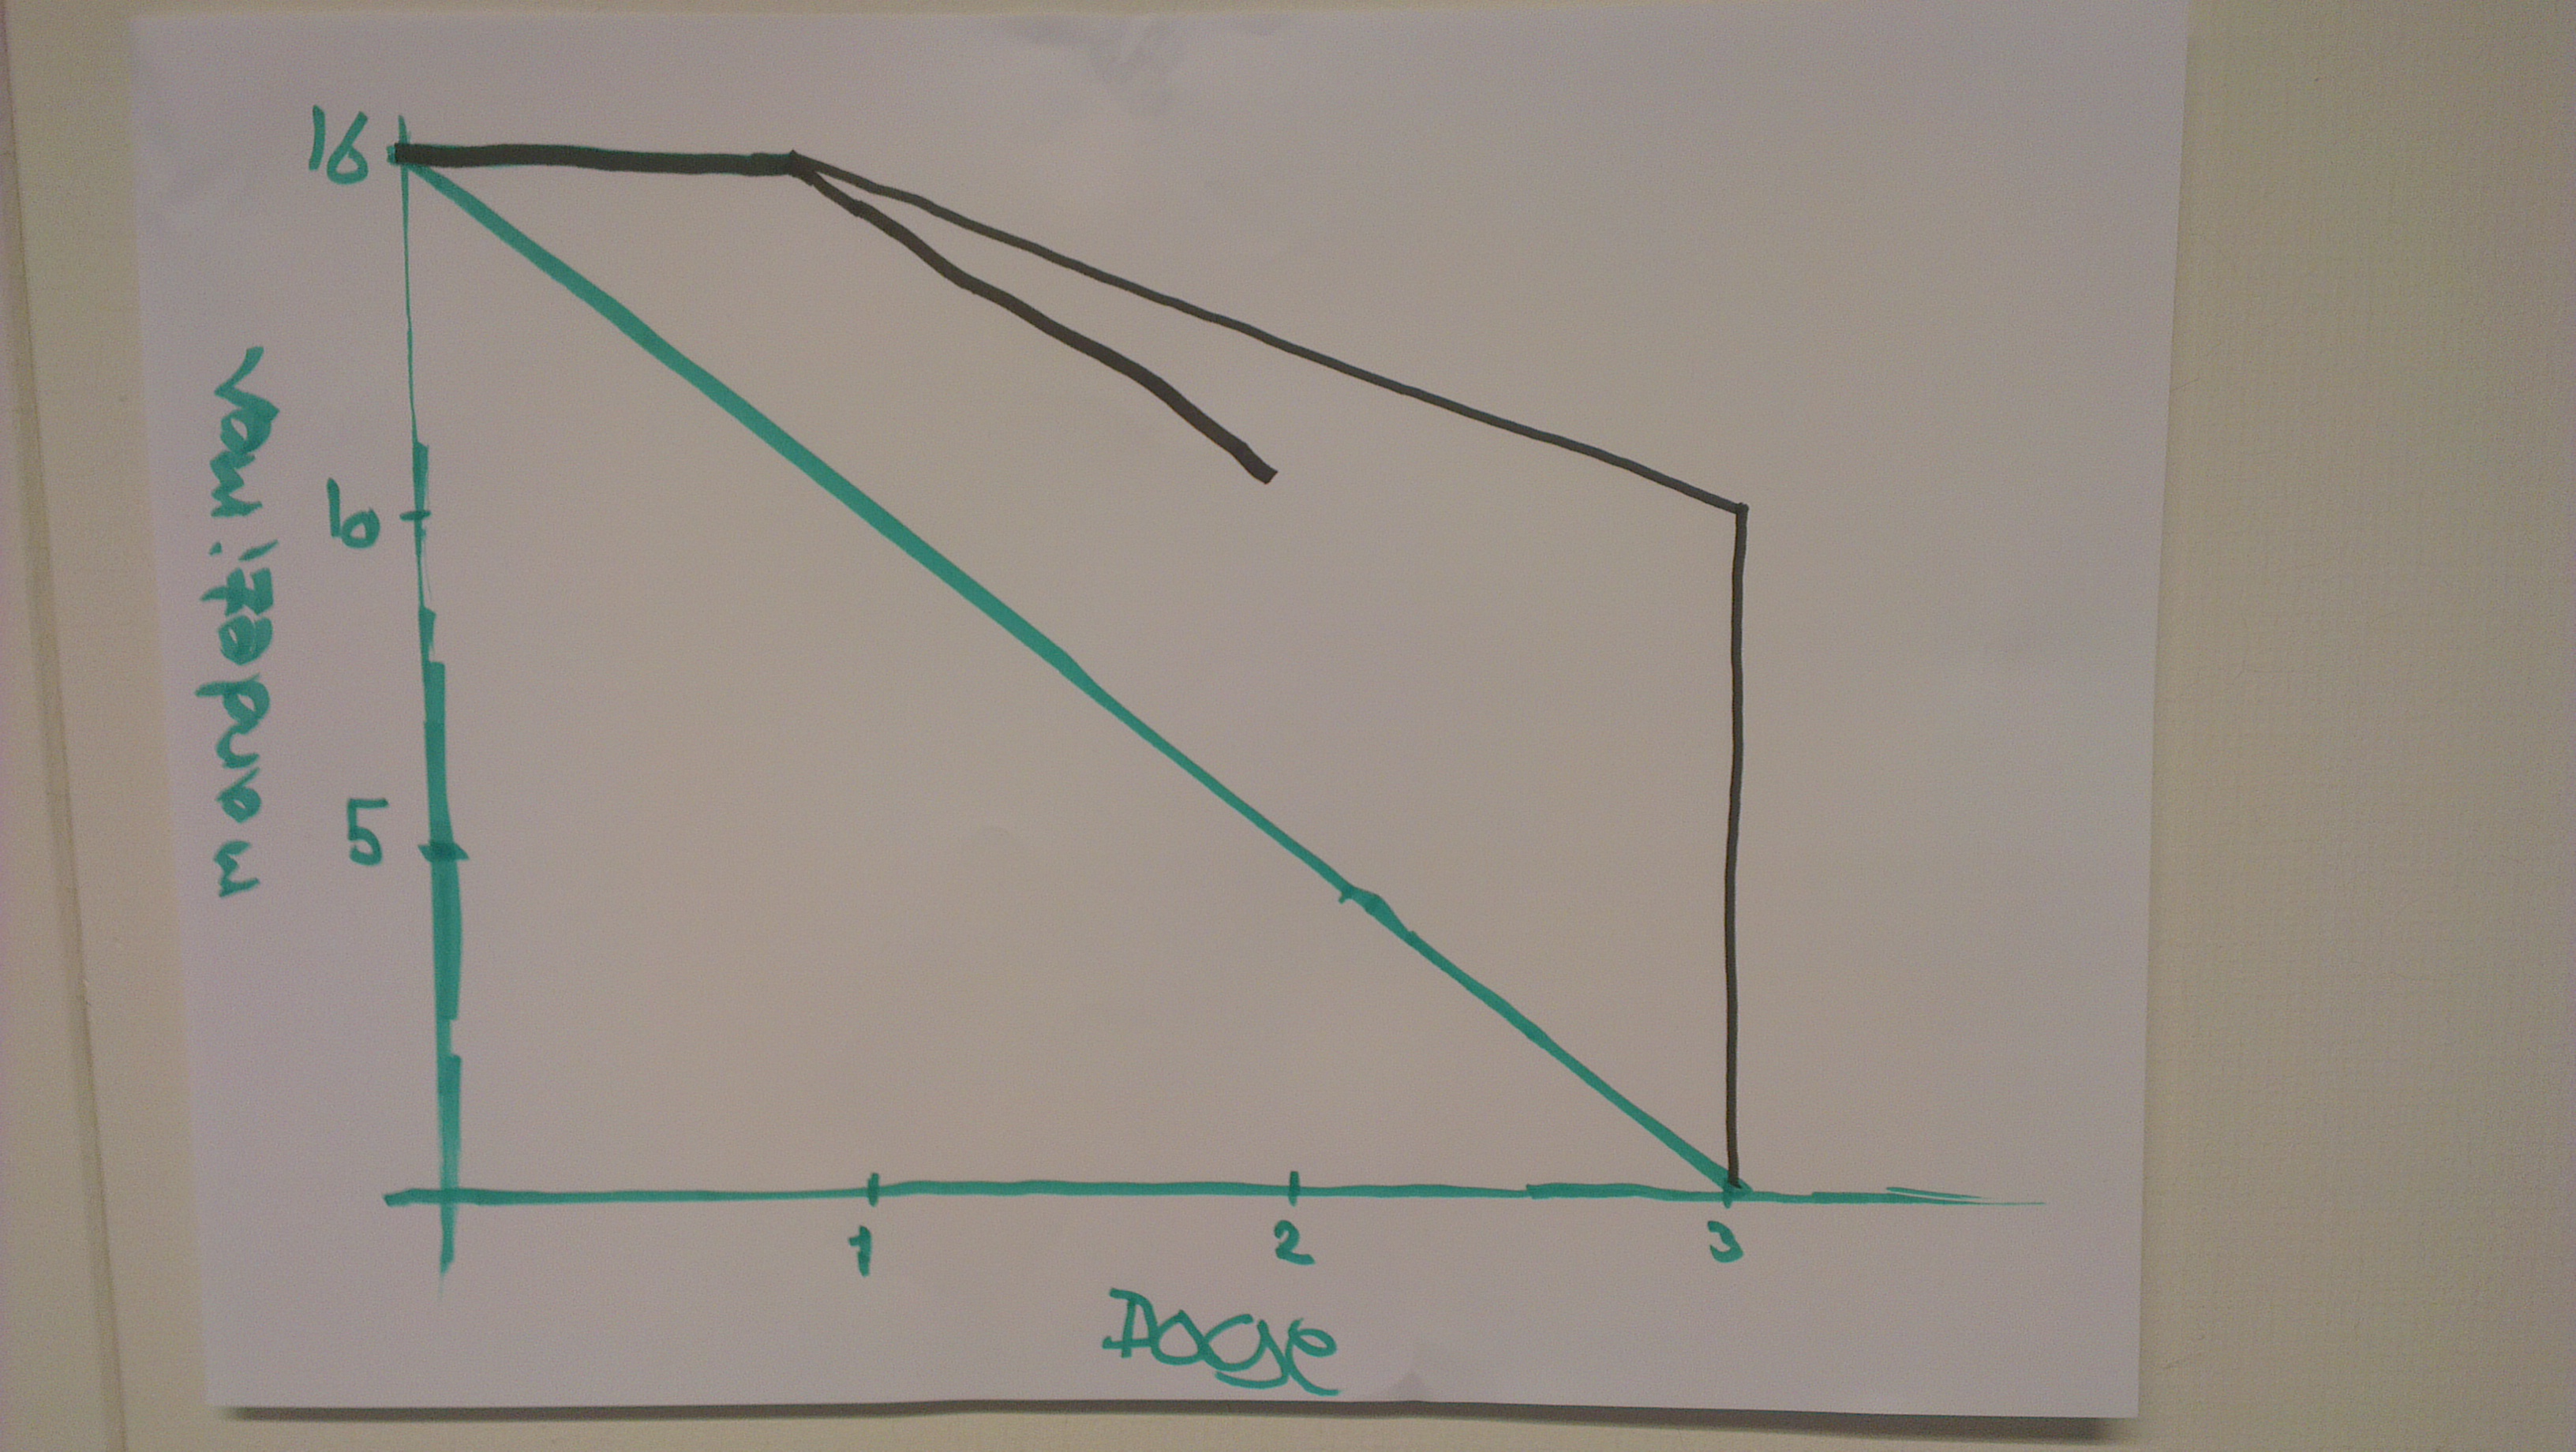
\includegraphics[scale=0.10]{includes/billeder/sprint3.jpg}
\caption{Sprint 3 burndown}
\label{fig:sprint3:burndown}
\end{center}
\end{figure}


\subsubsection*{Product backlog}
Til produkt backloggen har vi i dette sprint tilf�jet en user story med unit testing, samt at vi har �ndret prioriteten for diverse stories. \\

\begin{figure}[H]
\begin{center}
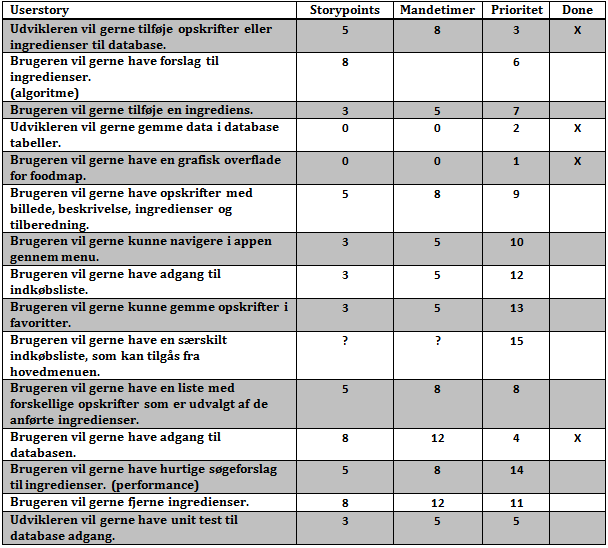
\includegraphics[scale=0.70]{includes/billeder/productbacklog_sprint3.png}
\caption{Sprint 3 produkt backlog}
\label{fig:sprint3:produktbacklog}
\end{center}
\end{figure}


\subsubsection*{Sprint backlog}
I sprint backloggen for dette sprint indg�r de to user stories:

\begin{figure}[H]
\begin{center}
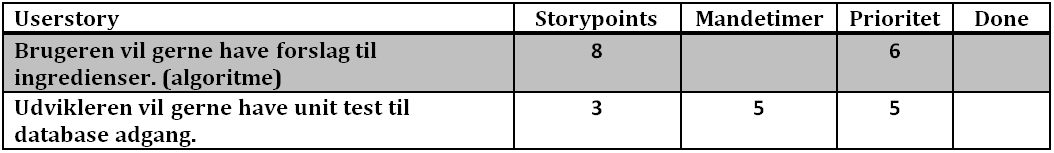
\includegraphics[scale=0.70]{includes/billeder/sprintbacklog_sprint3.png}
\caption{Sprint backlog}
\label{fig:sprint3:springbacklog}
\end{center}
\end{figure}

Ud af disse to stories fik vi lavet unit testene.


%\begin{itemize}
%\item Udvikleren vil gerne have unit test til database adgang.
%\item Brugeren vil gerne have forslag til ingredienser. (algoritme)
%\end{itemize}

\subsection*{Xp og scrum praktikker}
I sprint 3 benyttede vi fortsat XP praktikkerne: stand-up meeting, planning poker, par programmering, kollektivt kode ejerskab, kodestandarder, story board, metafor og simpelt design. 

\subsection*{Produkt review}
Til produkt reviewet viste vi vores foodmap gui med den funktionalitet vi havde n�et, samt vores unit test.


\subsection*{Retrospektive}
\textsf{Hvad gik godt:} \\
Vi fik lavet unit test og dermed fik vi lidt mere kvalitetssikring ind over vores projekt. \\

\textsf{Hvad gik mindre godt}
Alt for kort sprint med de 3 mandedage og derfor for meget pres p� for at have noget klar til reviewet. Is�r i forhold til at have noget visuelt klar at kunne vise. \\
Vi havde lidt meget parprogrammering pga. vores fokus p� test. 

\textsf{Hvad �ndrer vi til n�ste sprint:} \\
Sprint 3 var det sidste sprint vi havde tid til, men ellers vil vi fors�ge at lave l�ngere sprints fremadrettet, hvor vi arbejder lidt mere spredt.